%!TEX root = ../template.tex
%%%%%%%%%%%%%%%%%%%%%%%%%%%%%%%%%%%%%%%%%%%%%%%%%%%%%%%%%%%%%%%%%%%%
%% chapter3.tex
%% NOVA thesis document file
%%
%% Chapter with a short latex tutorial and examples
%%%%%%%%%%%%%%%%%%%%%%%%%%%%%%%%%%%%%%%%%%%%%%%%%%%%%%%%%%%%%%%%%%%%

\typeout{NT FILE chapter3.tex}%

\chapter{Dashboard Designer}
\label{cha:dashboard_designer}

%As ferramentas de análise e desenho de \textit{dashboards} não suportam devidamente o processo iterativo de design das mesmas. Neste capítulo, irá ser feita a introdução ao desenvolvimento de uma ferramenta baseada na linguagem \gls{IVML}, com o principal objetivo de culmatar a lacuna presente nas ferramentas mais utilizadas neste âmbito.

%Neste capítulo irá ser apresentado o meta-modelo desenvolvido. Este meta-modelo abrange não só a especificação da linguagem \gls{IVML} como toda a metodologia de suporte para a criação de \textit{dashboards}. De seguida, iram ser mencionados os protótipos de solução desenvolvidos, terminando pela listagem de requisitos e tecnologias que a solução desenvolvida necessita de ter presente.

As ferramentas existentes para a análise e desenho de \textit{dashboards} apresentam muitas limitações no que toca ao suporte de um processo iterativo de design, à exploração de alternativas e à recolha de \textit{feedack} por parte dos seus utilizadores. De forma a colmatar esta lacuna, este capítulo apresenta uma proposta inicial para o desenvolvimento de uma solução baseada na linguagem \gls{IVML}, criada para apoiar todo o processo de criação, prototipagem e documentação de \textit{dashboards} interativos.

Neste capítulo iram ser apresentados os meta-modelos desenvolvidos. Estes meta-modelos abrangem não só a especificação da linguagem \gls{IVML} como toda a metodologia de suporte para a criação de \textit{dashboards}. Os meta-modelos foram desenvolvidos em inglês, facilitando a compreensão, a partilha, e a possível integração futura com outras ferramentas e projetos internacionais. Ainda neste capítulo, iram ser mencionados os protótipos iniciais desenvolvidos, terminando pela listagem de requisitos e tecnologias que a solução necessita de ter presente.

\section{Abordagem} % (fold)
\label{sec:dashboard_abordagem}

Num primeiro plano, será feita uma adoção crítica da linguagem \gls{IVML}. A linguagem fornece uma base bastante consolidada para representar visualmente todos os elementos envolvidos no design de \textit{dashboards}, as suas interações, conjuntos de dados, e componentes de navegação. Neste sentido, foram desenvolvidos vários meta-modelos que combinam os princípios centrais da linguagem \gls{IVML} com a adição de uma componente analítica destinada a documentar os objetivos e propósitos que suportam a criação de cada \textit{dashboard}.

Relativamente ao processo de desenvolvimento, este será conduzido de forma incremental através da realização de \textit{sprints} semanais que, com o passar do tempo, irão resultar em diversas versões parciais da ferramenta. Esta abordagem irá permitir a realização de testes intermédios e recolher \textit{feedback} de forma contínua.

Para tornar a ferramenta orientada às necessidades dos seus utilizadores, é necessário ter em consideração certas tecnologias para tornar esta experiência o mais orientada para o seu público-alvo. O objetivo principal da criação de uma ferramenta no contexto da dissertação, é auxiliar o processo de conceção e design de \textit{dashboards}, facilitando o processo iterativo de comunicação entre todos os seus utilizadores.

De forma a tornar esta ferramenta orientada para as funcionalidades que tem de realizar, existem algumas características que se tornam imperativas de serem implementadas. Estas característica são:

\begin{itemize}
  \item Implementação de uma abordagem drag-and-drop.
  \item Integração de \textit{screenshots} reais para dar suporte aos elementos visuais.
  \item Capacidade de desenvolver várias opções de layout do dashboard.
  \item Implementação de atalhos como \textit{copy-past} e duplicação.
  \item Suporte para diferentes perfis de utilizador.
  \item Capacidade de representar os elementos segundo o meta-modelo apresentado em \ref{app:meta_modelo_app}.
  \item Capacidade de oferecer uma visão detalhada sobre cada elemento utilizado (tipo de visualização, dados utilizados, objetivos de visualização).
  \item Capacidade de simular o comportamento do \textit{dashboard}.
  \item Capacidade de recolher \textit{feedback} dos utilizadores sobre o \textit{dashboard} criado.
\end{itemize}

\section{Meta-modelo} % (fold)
\label{sec:meta_modelo}

%Especiificação do meta-modelo em detalhe
%No inicio falar sobre o metamodelo geral, o contexto e motivação que levaram à criação do meta-modelo
%Depois, criar várias secções que vão representar as diferentes componentes que o meta-modelo tem
Com o principal objetivo de apoiar os \textit{designers} no processo de conceção e prototipagem de \textit{dashboards} interativos, foi desenvolvido um meta-modelo que representa de forma estruturada a linguagem IVML e os diversos elementos envolvidos no processo de criação de \textit{dashboards}. Este meta-modelo irá ser utilizado como uma base conceptual para a ferramenta proposta, permitindo a representação tanto das componentes visuais e interativas de um \textit{dashboard}, como as suas componentes analíticas que sustentam a sua construção.

O desenho e estrutura do meta-modelo foi pensado para englobar não só os elementos visuais utilizados nas representações, como visualizações, interações, e \textit{tooltips}, mas também para incluir as fases iniciais que suportam o processo de criação de \textit{dashboards}, como a definição do âmbito de análise, a formulação de questões analíticas, e a identificação das perspetivas e objetivos de análise. Esta abordagem mais abrangente de elementos tem como objetivo mostrar que o processo de \textit{design} de \textit{dashboards} interativos não se foca apenas na representação gráfica dos seus elementos, mas também na definição da componente analítica que justifica a sua criação.

É apresentado em apêndice o meta-modelo completo, que englaba todas as diferentes componentes numa só representação (ver apêndice \ref{app:meta_modelo_app}). Nas secções seguintes, vai ser feita a descrição detalhada das diferentes componentes que definem o meta-modelo. Esta abordagem de separação do meta-modelo em diferentes componentes de menor amplitude facilita não só a sua apresentação, como a sua compreensão para um público-alvo menos experiente na área.

\subsection{Componente Analítica e Estrutural} % (fold)
\label{sub:anal_struct_comp}

Nesta secção serão exploradas em detalhe as duas componentes centrais que definem o meta-modelo: a componente analítica e a componente estrutural. A organização conceptual destas componentes pode ser observada na Figura \ref{fig:comp_anal_struct}. Adicionalmente, a componente analítica inclui exemplos integrados na sua representação, baseados em casos concretos retirados da dissertação de Ana Milroy \cite{milroy2025}, de forma a facilitar a interpretação da mesmo.

A componente analítica tem como principal objetivo representar o processo inicial de definição conceptual e estratégica que orienta a criação dos diferentes \textit{dashboards}. Esta componente é composta por diferentes entidades que, de forma conjunta, tornam o processo de conceptualização possível. Cada entidade presente na componente descrita desempenha um papel fundamental para a correta implementação dos conceitos analíticos necessário para a conceção de uma \textit{dashboard}. O processo tem início na entidade \textbf{Analysis Scope}, que define o âmbito geral da análise e estabelece o contexto onde se vão inserir os \textit{dashboards} a desenvolver. Esta entidade constitui o ponto de partida de todo o raciocínio analítico, uma vez que é através da estipulação do âmbito que se definem os restante elementos. Associada ao âmbito, surge a entidade de \textbf{Datum}, que, em conjunto com a entidade \textbf{Data Collection} definem o conjunto de dados disponíveis a serem utilizados para responder às diferentes necessidades analíticas. A entidade \textbf{Question Collection} agrupa o conjunto de questões analíticas que se pretendem ver respondidas com a implementação dos diferentes \textit{dashboards}. Estas questões são formuladas com base no âmbito de análise em que estão inseridas e devem estar alinhadas com as necessidades dos utilizadores. Dentro de cada âmbito podem ser definidos diferentes \textbf{Analysis Themes}, que representam as áreas específicas no âmbito que pretendemos analisar. Cada tema de análise pode ser analisado sob diferentes \textbf{Analysis Perspective} que se referem a diferentes formas de analisar e representar os temas a que estão associados. Por fim, cada perspetiva está associada a um ou mais \textbf{Analysis Objective}, que definem as metas que se pretendem vir a ser atingidas através das diferentes visualizações que irão compor os \textit{dashboards}.

A segunda componente representada no diagrama é a componente estrutural, cujo principal objetivo é representar os diferentes elementos visuais e interativos que vão ser utilizados na representação dos diferentes \textit{dashboards} a desenvolver. A entidade que desempenha um papel central nesta componente é a \textbf{Dashboard}, responsável por agregar todos os elementos que compôem a interface visual. Cada \textit{dashboard} pode integrar múltiplas entidades \textbf{Visualization}, que correspondem às representações gráficas dos dados a serem analisados (como gráficos, mapas ou tabelas). Uma visualização pode estar associada a zero o mais entidades \textbf{Caption}, que representam a legenda da informação que está a ser mostrada nas diferentes visualizações. Cada visualização pode estar associada a zero ou mais entidades \textbf{Tooltip}, estas entidades fornecem informação adicional ao utilizador sobre um ou mais elementos presentes na visualização. A entidade \textbf{Placeholder} pode estar associada tanto à visualização como ao próprio \textit{dashboard}, e serve para representar componentes estáticas como imagens ou títulos. Esta entidade contribui para estruturar o \textit{display} da interface, sem sobrecarregar o utilizador com informação analítica. Por fim, é introduzida a entidade \textbf{InteractionComp}, uma classe abstrata que agrega diferentes tipos de componentes interativos, com comportamentos distintos. A primeira entidade é \textbf{Button}, esta entidade é utilizada para ilustrar botões acionávies responsávies por executar ações específicas. A segunda entidade é \textbf{Parameter}, usada quando se pretende introduzir parâmetros que influenciam diretamente o conteúdo a ser mostrado. Finalmente, é introduzida a entidade \textbf{Filter},destina à representação de filtros aplicáveis a uma ou mais visualizações, permitindo refinar os dados exibidos conforme os critérios definidos pelo utilizador.

%aqui não esquecer de citar a tese da ana mais uma vez e referenciar a utilização de exemplos para facilitar a análise do diagrama
Como é possível observar na Figura \ref{fig:comp_anal_struct}, são estabelecidas ligações diretas de dependência e agregação entre entidades da componente estrutural e entidades da componente analítica, sendo esta a razão pela qual estas componentes são apresentadas de forma simultânea e não de forma separada. Estas ligações entre componentes descrevem o comportamento e relação funcional que estas componentes têm em comum. Um exemplo destas ligações é a relação entre a entidade \textbf{Analysis Perspective} e a entidade \textbf{Dashboard}. Como é descrito anteriormente, cada tema de análise pode englobar uma ou mais perspetivas de análise, sendo que estas perspetivas de análise são representadas visualmente através da criação de diferentes tipos de \textit{dashboard}. Da mesma forma, a entidade \textbf{Analysis Objective} está diretamente ligada à entidade \textbf{Visualization}. Cada perspetiva de análise pode agregar um ou mais objetivos de análise, sendo que estes objetivos são respondidos através da criação de diferentes tipos de visualização. Estas ligações entre entidades são a ponte que estabelece a ligação entre a componente analítica e estrutural, dando contexto às diferentes componentes visuais implementadas nas representações.

\begin{figure}[htbp]
  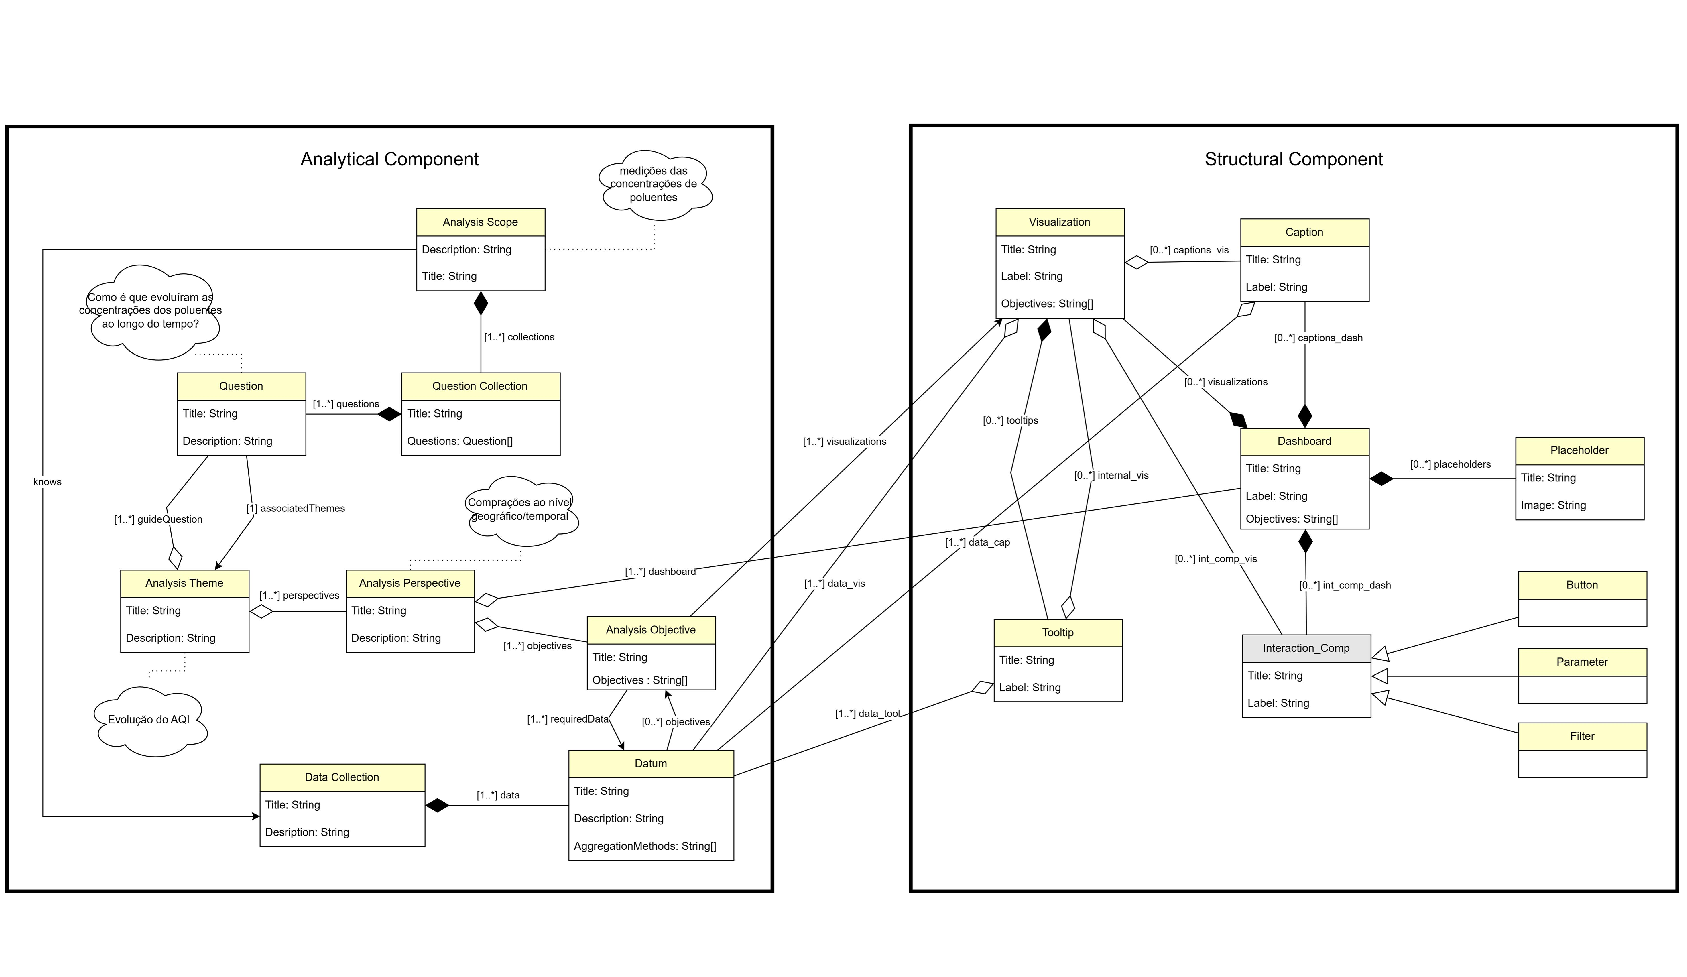
\includegraphics[width=\textwidth]{meta_modelo/compAnlyticalStructural_cropped}
  \centering
  \caption{Componente Analítica e Estrutural do meta-modelo.}
  \label{fig:comp_anal_struct}
\end{figure}

\subsection{Atributos dos Dados e Atributos Visuais} % (fold)
\label{sub:data_vis_attr}

Depois de definirmos a componente analítica e a componente estrutural, isto é, depois de definirmos o que será analisado e como iremos estruturar o \textit{dashboard}, é essencial definirmos como é que os dados vão ser representados visualmente. É neste contexto que entra a componenente de dados e atributos visuais, esta componente tem como principal objetivo estabelecer a ligação entre os dados e os elementos gráficos que os representam. Esta componente encontra-se representada na Figura \ref{fig:comp_data_vis}.

A componente de dados e atríbutos visuais tem como principal objetivo a representação gráfica dos dados de forma a torná-los de fácil compreensão. Desta forma, as duas entidades que apresentam um papel central nesta componente são: \textbf{Visualization}, a entidade responsável por fazer a conversão direta dos dados em representações visuais de fácil compreensão, e \textbf{Datum}, a entidade que representa os dados a serem utilizados nas diferentes visualizações. Cada visualização pode representar os dados através de diferentes tipos de representações gráficas, é aqui que entra a classe abstrata \textbf{Graph Type}, a classe que agrupa todos os tipos de representação gráfica que uma visualização pode tomar (como gráficos de barras, linhas, mapas, entre outros). Para ajudar a representação, as visualizações podem ter associadas \textbf{Visual Variables} e \textbf{Captions}. As variávies visuais são utilizadas para distinguir métricas diferentes dentro de uma mesma visualização, através da utilização de elementos como cor, forma ou tamanho. As legendas, por sua vez, servem para fornecer contexto à informação apresentada nas diferentes visualizações. Já mencionadas na componente estrutural, as legendas são cruciais para garantir que o utilizador compreenda completamente o que está a ser mostrado.

\begin{figure}[htbp]
  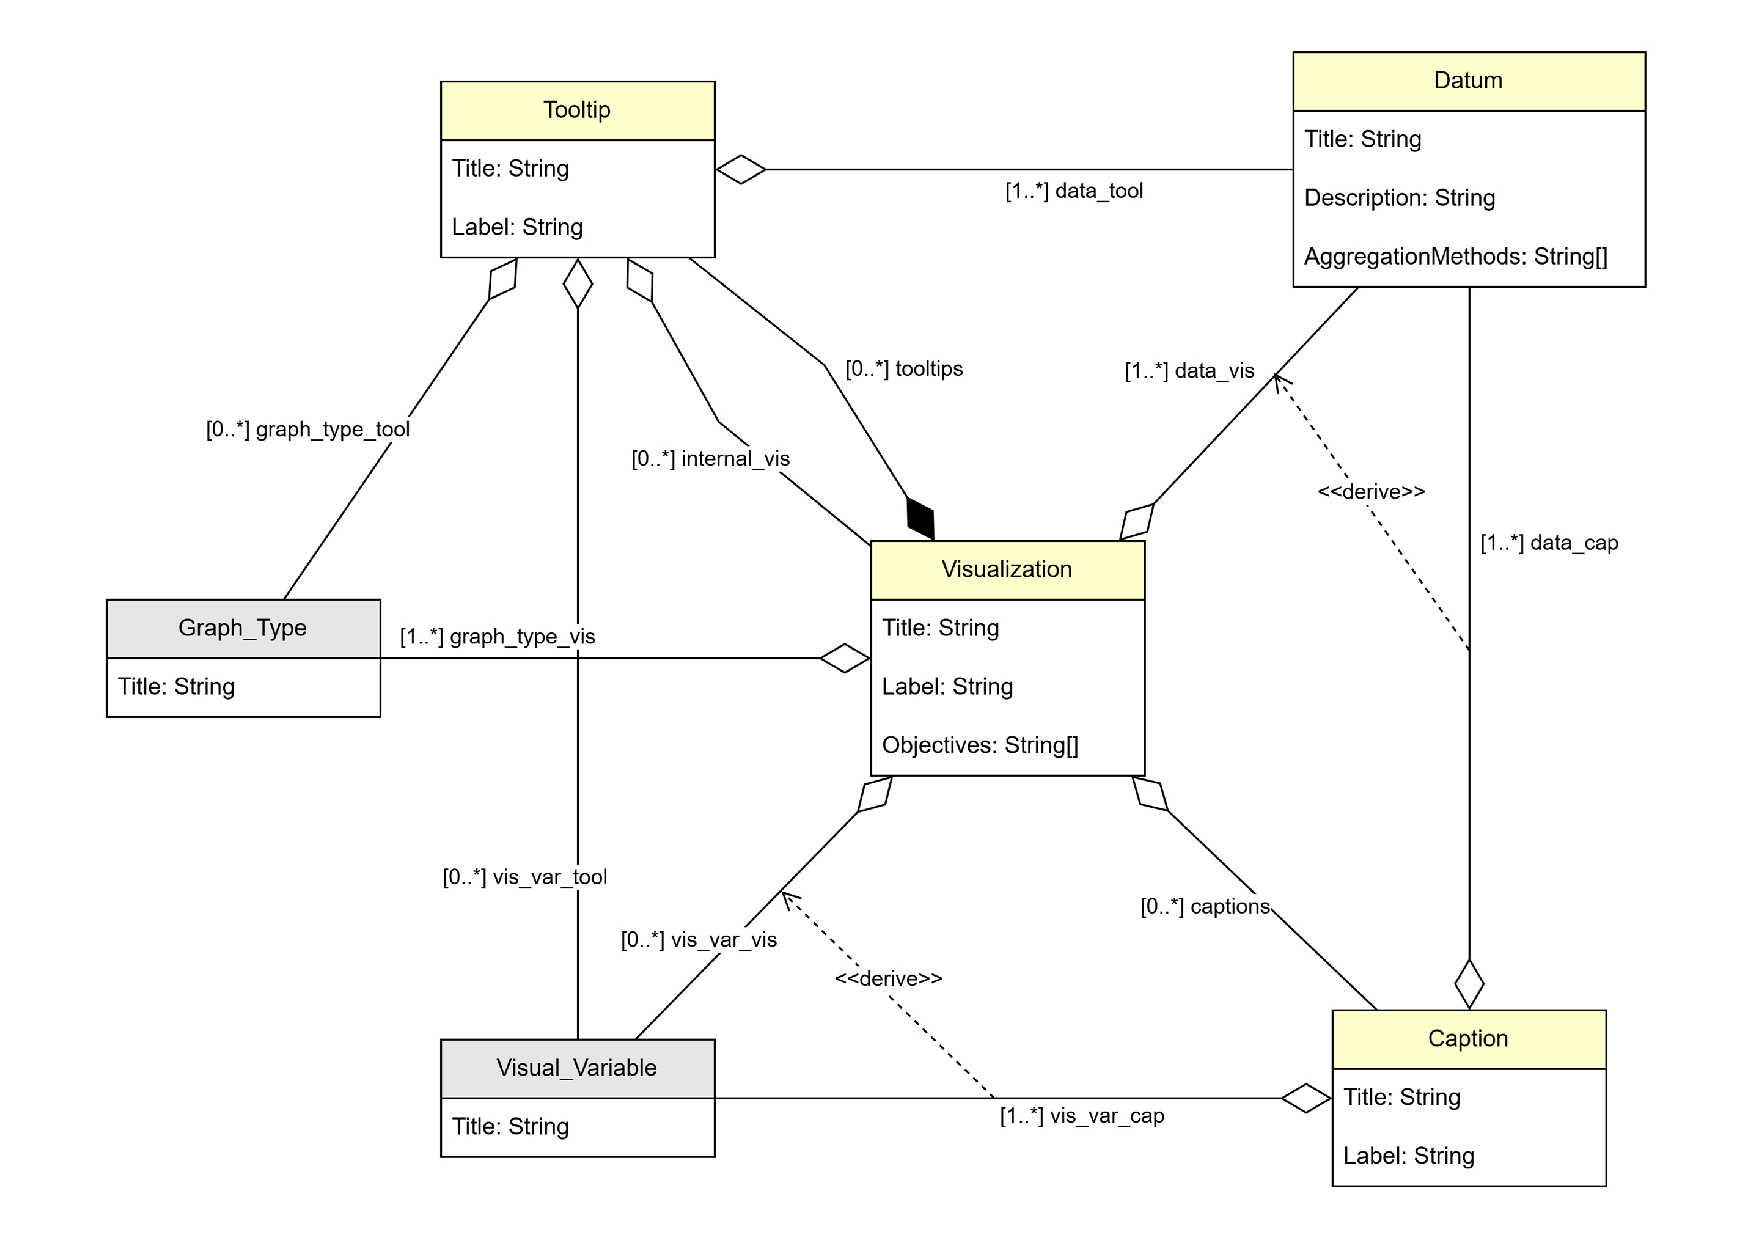
\includegraphics[width=\textwidth]{meta_modelo/dataVis}
  \centering
  \caption{Componente de Dados e Atríbutos Visuais do meta-modelo.}
  \label{fig:comp_data_vis}
\end{figure}

\subsection{Componente de Interações} % (fold)
\label{sub:int_diagram}

A componente de interação permite representar os diferentes elementos responsáveis por promover a interatividade entre o utilizador e o \textit{dashboard}. É através desta componente que é possível tranformar um \textit{dashboard} estático e pouco interativo numa solução dinâmica, interativa e de fácil utilização, onde é dado ao utilizador a possibilidade de navegar por diferentes prespetivas e compreender melhor as relações que as diferentes componentes estabalecem entre si. A representação visual desta componente encontra-se ilustrada na Figura \ref{fig:interaction}.

Esta componente é modelada a partir da classe abstrata \textbf{Interaction Comp}, que representa os elementos que introduzem comportamento no \textit{dashboard}, nomeadamente \textbf{Button}, \textbf{Parameter}, e \textbf{Filter}. Estas entidades estão sempre associadas a um \textbf{Interaction Type}, que define a forma como a interação vai ser desencadeada, por exemplo, através de um \textbf{Click} ou de um \textbf{Hover}. De entre as três entidades de interação, os parâmetros e filtros desempenham um papel direto na manipulação dos dados. Estas duas entidades são ligadas à entidade \textbf{Data Action} que representa a ação que será aplicada sobre os dados. Cada ação é classificada segundo um \textbf{Action Type}, determinando o efeito que terá na visualização dos dados, podendo este ter efeito de \textbf{Highlight} ou de \textbf{Filtering}. Estes tipos de ações resultam num impacto direto sobre as várias entidades visuais, como \textbf{Visualization}, \textbf{Caption}, e \textbf{Dashboard}, modificando a informação apresentada ao utilizador com base nas diferentes interações realizadas. A entidade \textbf{Datum}, para além de representar os diferentes dados presentes nas diferentes entidades, esta entidade pode ser usada para ativar \textbf{Tooltips} através de um tipo de interação associado. Desta forma, a componente de interação desempenha um papel essencial no reforço da experiência analítica do utilizador. 
%A classe abstracta \textbf{Interaction Comp} representa esta componente, ou seja, ela representa as diferentes entidades que dão comportamente e vida de forma direta aos \textit{dashboards}, sendo estas \textbf{Button}, \textbf{Parameter}, e \textbf{Filter}. Estas entidades precisam sempre de estar associadas a um \textbf{Interaction Type}, que representa o tipo de interação que ativa estas entidades, podendo estas ser \textbf{Hover} ou \textbf{Click}. De as três entidades da componente de interação, as entidades de parâmetro e filtro são responsáveis por fazer alterações diretas na entidade \textbf{Data} através da entidade \textbf{Data Action}. A entidade de ação de dados encontr-se sempre associada a uma \textbf{Action Type} que define o tipo de ação que é aplicada sobre os dados, podendo esta ser \textbf{Filtering} ou de \textbf{Highlight}. Estes tipos de interação têm efeitos diretos nas diferentes \textbf{Visualizations}, \textbf{Captions}, e \textbf{Dashbaords}, atrvés da alteração da informação a ser mostrada por estas diferentes entidades.

\begin{figure}[htbp]
  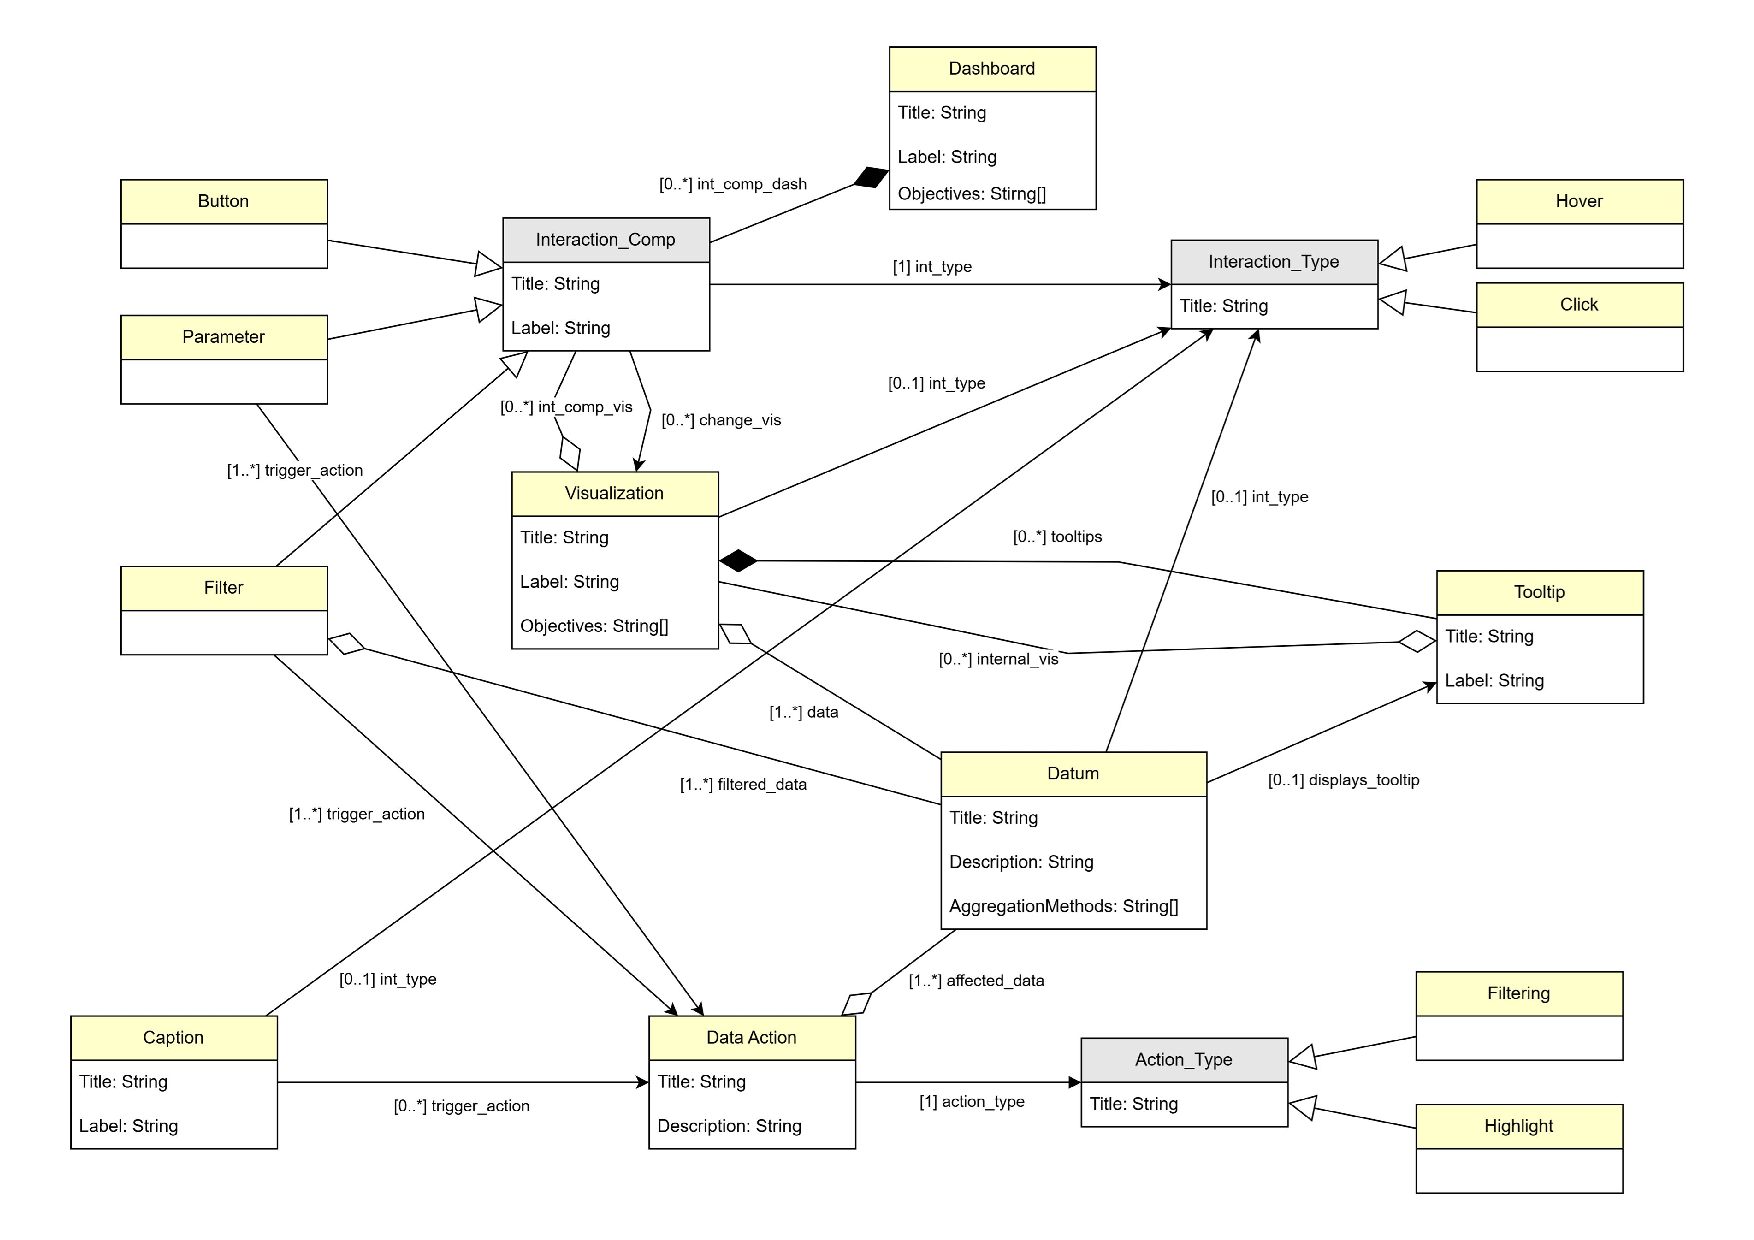
\includegraphics[width=\textwidth]{meta_modelo/interaction}
  \centering
  \caption{Componente de Interação do meta-modelo.}
  \label{fig:interaction}
\end{figure}

\subsection{Componente de Navegação} % (fold)
\label{sub:nav_diagram}

A última componente criada no âmbito do meta-modelo é a componente de navegação. Esta componente representa as diferentes formas que o utilizador possui de forma a mudar de contexto analítico através de navegação entre outros \textit{dashboards} ou através de ligações externas. A representação visual desta componente encontra-se ilustrada na Figura \ref{fig:navigation}.

A entidade central neste tipo de componente é a classe abstrata \textbf{Navegation Comp}, que representa os diferentes tipos de navegação possíveis. Através desta classe, é possível definir dois comportamentos distintos:

\begin{itemize}
    \item \textbf{Dashboard Nav} que representa a navegação interna entre \textit{dashboards};
    \item \textbf{Nav Link} que representa a navegação externa, como por exemplo, para páginas web;
\end{itemize}

De forma semelhante à componente de interação, a componente de navegação está sempre associada a um \textbf{Interaction Type} que define a forma como a navegação vai ser desencadeada - nomeadamenta por um \textbf{Click} ou por um \textbf{Hover}. Esta componente de navegação pode estar associada a diferentes tipos de elementos visuais, tais como, \textbf{Button} e \textbf{Datum}. Esta integração permite que o utilizador integre facilmente mecanismos de navegação nas diferentes representações visuais, tornando a navegação mais simples e adaptada às necessidades do utilizador.

\begin{figure}[htbp]
  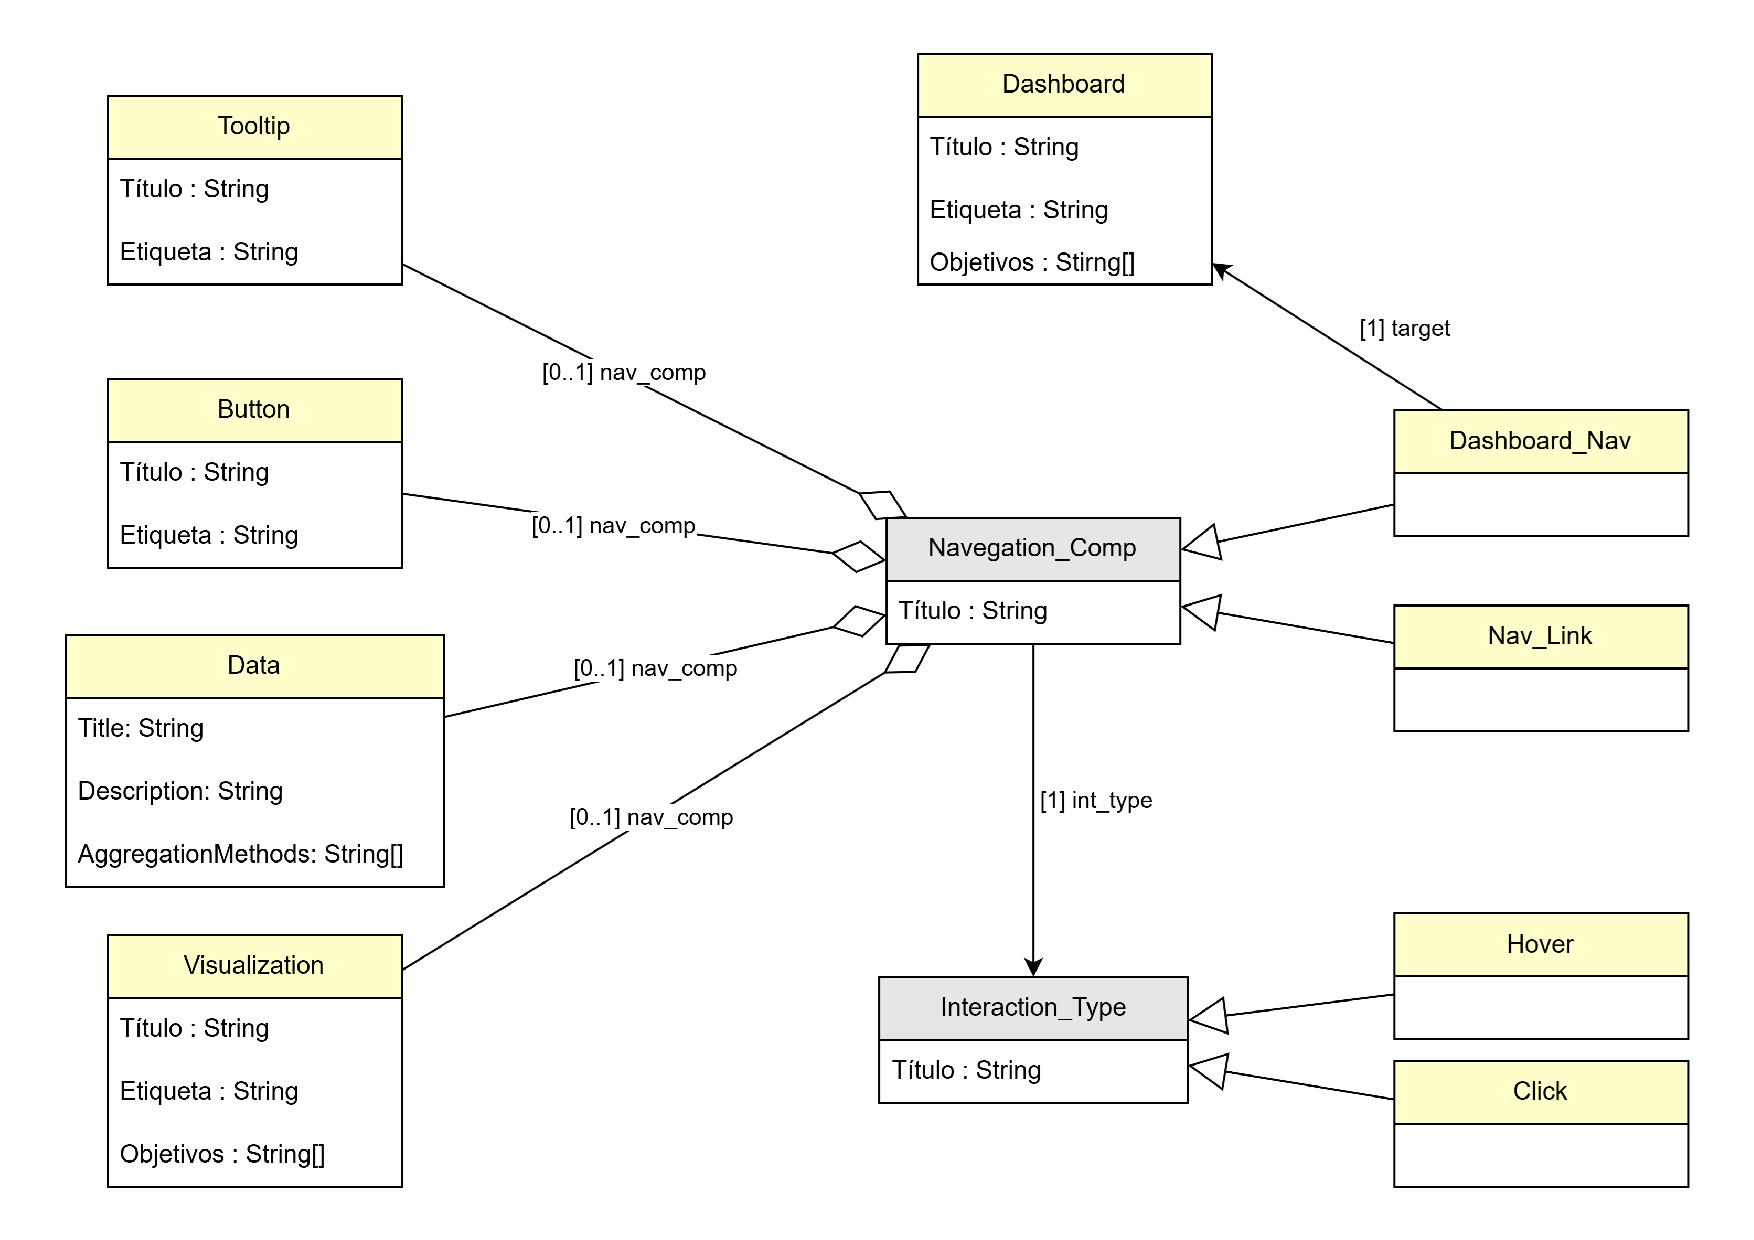
\includegraphics[width=\textwidth]{meta_modelo/navigation}
  \centering
  \caption{Componente de Navegação do meta-modelo.}
  \label{fig:navigation}
\end{figure}

\section{Protótipo Preliminar Desenvolvido} % (fold)
\label{sec:prototipo_preliminar}

%Ver melhor o titulo mas aqui é onde vou falar sobre os prototipos feitos numa fase inicial onde a ferramenta apenas se ia centrar no IVML
%introdução, dizer que meti em anexo o protótipo, dizer que foi numa fase inicial
Para o desenvolvimento de qualquer ferramenta, é crucial que sejam implementados protótipos representativos, quer para representar as diferentes componentes visuais que a mesma terá, quer para representar as componentes técnicas.

Numa fase inicial do desenvolvimento da dissertação, foi implementado um protótipo da ferramenta em Figma \cite{figma} baseada na linguagem \gls{IVML}. Este protótipo tinha como principal objetivo representar todas as componentes visuais e técnicas que a solução final iria possuir. Uma vez que este protótipo foi realizado numa fase inicial, o mesmo já não se encontra de acordo com a estrutura e organização do meta-modelo desenvolvido e mencionado na secção \ref{sec:meta_modelo}. O protótipo desenvolvido é apresentado no apêndice \ref{app:prototipo_inicial}. Como é possível observar, o mesmo apenas representa as diferentes componentes que a linguagem \gls{IVML} possuiu, ignorando toda a componente analítica que é necessária para a criação de diferentes \textit{dashboards} interativas.

\begin{comment}

\section{Requisitos da ferramenta} % (fold)
\label{sec:requisitos}

%Tecnologias e requisitos que eu já sei que a ferramenta terá de ter
Para tornar a ferramenta orientada às necessidades dos seus utilizadores, é necessário ter em consideração certas tecnologias para tornar esta experiência o mais orientada para o seu público-alvo. O objetivo principal da criação de uma ferramenta no contexto da dissertação, é auxiliar o processo de conceção e design de \textit{dashboards}, facilitando o processo iterativo de comunicação entre todos os seus utilizadores.

De forma a tornar esta ferramenta orientada para as funcionalidades que tem de realizar, existem algumas características que se tornam imperativas de serem implementadas. Estas característica são:

\begin{itemize}
  \item Implementação de uma abordagem drag-and-drop.
  \item Integração de \textit{screenshots} reais para dar suporte aos elementos visuais.
  \item Capacidade de desenvolver várias opções de layout do dashboard.
  \item Implementação de atalhos como \textit{copy-past} e duplicação.
  \item Suporte para diferentes perfis de utilizador.
  \item Capacidade de representar os elementos segundo o meta-modelo apresentado em \ref{app:meta_modelo_app}.
  \item Capacidade de oferecer uma visão detalhada sobre cada elemento utilizado (tipo de visualização, dados utilizados, objetivos de visualização).
  \item Capacidade de simular o comportamento do \textit{dashboard}.
  \item Capacidade de recolher \textit{feedback} dos utilizadores sobre o \textit{dashboard} criado.
\end{itemize}

\end{comment}